\documentclass[margin=3mm]{standalone}
\usepackage{tikz}
\usetikzlibrary{arrows.meta}

\begin{document}
    \thispagestyle{empty}

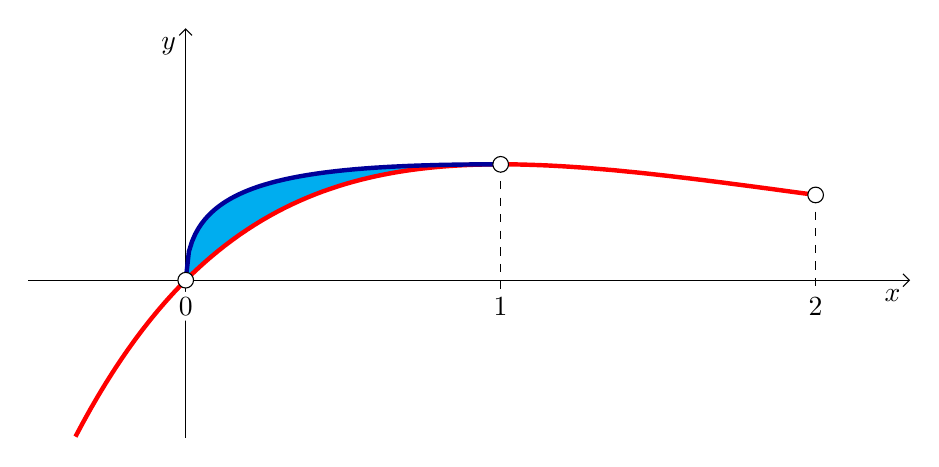
\begin{tikzpicture}[scale=4,
arr/.style = {-Straight Barb},
wdt/.style = {circle, draw, solid, fill=white, inner sep=2pt},
tck/.style = {rounded corners, inner sep=2pt, fill=white, anchor=north}
                    ]
% axis
\draw[arr] (-0.5,0) -- (2.3,0) node[below left]    {$x$};
\draw[arr] (0,-0.5) -- (0,0.8) node[below left]    {$y$};
% fill between curves
\fill[cyan] plot[samples at={0,0.01,...,0.2,0.3,...,1}] (\x,{sqrt(\x)*e^(-sqrt(\x))}) --
            plot[samples=100, domain=1:0] (\x,{\x*e^(-\x)});
% curves
\draw[ultra thick, samples=100, red] plot[domain=-0.35:2] (\x,{\x*e^(-\x)});
\draw[ultra thick, samples=100, blue!60!black]  plot[domain=-0:1] (\x,{sqrt(\x)*e^(-sqrt(\x))});
% circles + dashed line
    \foreach \x in {0,1,2}
\draw[dashed]  (\x,{\x*e^(-\x)})  node (\x) [wdt] {} -- (\x |- 0,-1pt) node[tck] {\x};
\end{tikzpicture}

\end{document}